\documentclass[11pt]{article}
\usepackage[margin=1in]{geometry}
\usepackage[T1]{fontenc}
\usepackage{tikz}
\usepackage[american]{circuitikz}
\usepackage{longtable}
\usepackage{hyperref}
\title{schmitt\_trigger}
\author{Generated by mixedsig2cad}
\date{\today}
\begin{document}
\maketitle
\section{Readable Circuit}
\begin{circuitikz}[american voltages, scale=1, transform shape]
  \draw (16.89,-11.81) to[R,l={100k},t={R3}] (18.16,-11.81);
  \draw (14.10,-8.51) to[R,l={100k},t={R1}] (14.10,-9.78);
  \draw (8.00,-9.27) to[V,l={PWL(0 0 1m 5 2m 0)},t={VIN}] (8.00,-10.80);
  \draw (8.00,-13.21) to[V,l={DC 2.5},t={VREF}] (8.00,-14.73);
  \draw (14.10,-9.78) to[R,l={100k},t={R2}] (14.10,-11.05);
  \draw (8.00,-5.21) to[V,l={DC 5},t={VCC}] (8.00,-6.73);
  \draw (16.51,-9.02) rectangle (17.53,-10.03);
  \node[font=\scriptsize,align=center] at (17.02,-9.53) {XU1\\OPCMP};
  \draw (16.26,-9.78) -- (16.51,-9.78);
  \draw (16.26,-9.27) -- (16.51,-9.27);
  \draw (17.78,-9.53) -- (17.53,-9.53);
  \draw (16.76,-8.76) -- (16.76,-9.02);
  \draw (16.76,-10.29) -- (16.76,-10.03);
  \node[font=\scriptsize,anchor=south] at (8.00,-4.95) {VCC};
  \draw (8.00,-8.00) node[ground] {};
  \node[font=\scriptsize,anchor=south] at (16.76,-9.02) {VCC};
  \draw (14.10,-11.94) node[ground] {};
  \draw (16.76,-11.05) node[ground] {};
  \draw (8.00,-11.94) node[ground] {};
  \draw (8.00,-16.00) node[ground] {};
  \draw (14.10,-11.05) -- (14.10,-11.94);
  \draw (8.00,-6.73) -- (8.00,-8.00);
  \draw (16.76,-10.29) -- (16.76,-11.05);
  \draw (8.00,-14.73) -- (8.00,-16.00);
  \draw (8.00,-10.80) -- (8.00,-11.94);
  \draw (8.00,-5.21) -- (8.00,-4.95);
  \draw (16.76,-8.76) -- (16.76,-9.02);
  \draw (8.00,-9.27) -- (8.00,-8.89);
  \draw (15.75,-9.27) -- (16.26,-9.27);
  \draw (18.16,-11.81) -- (18.54,-11.81);
  \draw (18.54,-11.81) -- (18.54,-9.53);
  \draw (17.78,-9.53) -- (18.54,-9.53);
  \draw (16.89,-11.81) -- (14.73,-11.81);
  \draw (14.73,-11.81) -- (14.73,-9.78);
  \draw (14.73,-9.78) -- (16.26,-9.78);
  \draw (14.73,-9.78) -- (14.10,-9.78);
  \draw (8.00,-13.21) -- (8.00,-12.83);
  \fill (14.73,-9.78) circle (1.2pt);
  \fill (14.10,-9.78) circle (1.2pt);
  \node[font=\scriptsize] at (17.53,-11.43) {R3};
  \node[font=\scriptsize] at (17.53,-12.19) {100k};
  \node[font=\scriptsize] at (14.61,-9.40) {R1};
  \node[font=\scriptsize] at (13.59,-9.40) {100k};
  \node[font=\scriptsize] at (7.62,-9.14) {VIN};
  \node[font=\scriptsize] at (6.22,-10.54) {PWL(0 0 1m 5 2m 0)};
  \node[font=\scriptsize] at (7.75,-13.08) {VREF};
  \node[font=\scriptsize] at (8.38,-14.86) {DC 2.5};
  \node[font=\scriptsize] at (13.59,-10.67) {R2};
  \node[font=\scriptsize] at (13.59,-10.41) {100k};
  \node[font=\scriptsize] at (7.62,-6.86) {VCC};
  \node[font=\scriptsize] at (6.98,-6.48) {DC 5};
  \node[font=\scriptsize] at (17.02,-10.29) {XU1};
  \node[font=\scriptsize] at (17.27,-8.76) {OPCMP};
  \node[font=\scriptsize] at (8.00,-4.45) {VCC};
  \node[font=\scriptsize] at (8.00,-8.51) {GND};
  \node[font=\scriptsize] at (14.10,-8.51) {vref};
  \node[font=\scriptsize] at (16.76,-8.51) {VCC};
  \node[font=\scriptsize] at (14.10,-12.45) {GND};
  \node[font=\scriptsize] at (15.75,-9.27) {vin};
  \node[font=\scriptsize] at (16.76,-11.56) {GND};
  \node[font=\scriptsize] at (8.00,-12.45) {GND};
  \node[font=\scriptsize] at (8.00,-8.89) {vin};
  \node[font=\scriptsize] at (8.00,-12.83) {vref};
  \node[font=\scriptsize] at (8.00,-16.51) {GND};
  \node[font=\scriptsize] at (18.54,-9.53) {vout};
  \node[font=\scriptsize] at (16.26,-9.78) {vplus};
\end{circuitikz}
\section{Literal KiCad Reference}
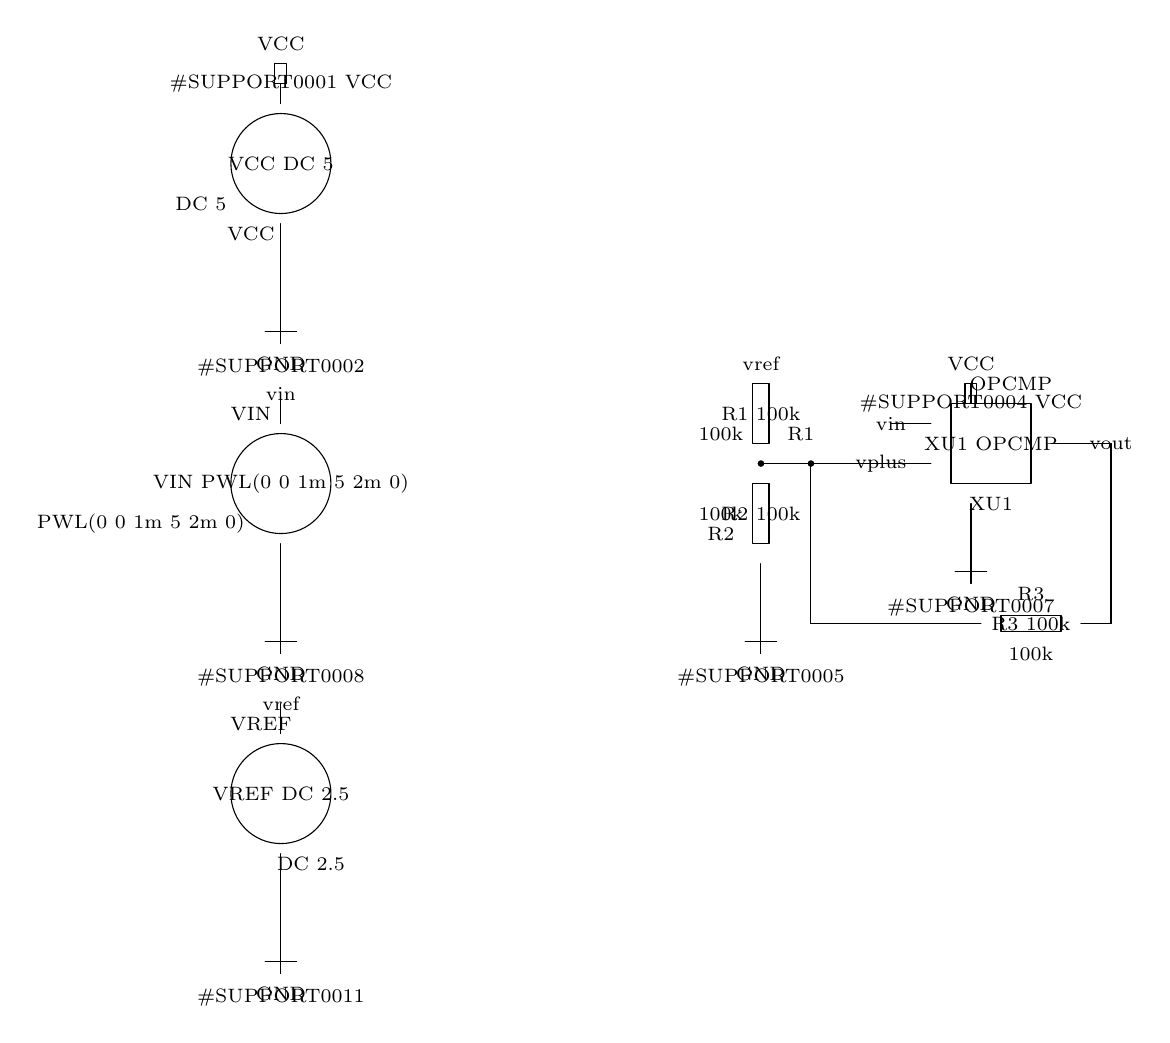
\begin{tikzpicture}[x=0.1cm,y=-0.1cm,line cap=round,line join=round]
  \draw (140.97,110.49) -- (140.97,119.38);
  \draw (80.01,67.31) -- (80.01,80.01);
  \draw (167.64,102.87) -- (167.64,110.49);
  \draw (80.01,147.32) -- (80.01,160.02);
  \draw (80.01,107.95) -- (80.01,119.38);
  \draw (80.01,52.07) -- (80.01,49.53);
  \draw (167.64,87.63) -- (167.64,90.17);
  \draw (80.01,92.71) -- (80.01,88.90);
  \draw (157.48,92.71) -- (162.56,92.71);
  \draw (181.61,118.11) -- (185.42,118.11);
  \draw (185.42,118.11) -- (185.42,95.25);
  \draw (177.80,95.25) -- (185.42,95.25);
  \draw (168.91,118.11) -- (147.32,118.11);
  \draw (147.32,118.11) -- (147.32,97.79);
  \draw (147.32,97.79) -- (162.56,97.79);
  \draw (147.32,97.79) -- (140.97,97.79);
  \draw (80.01,132.08) -- (80.01,128.27);
  \fill (147.32,97.79) circle (1.2pt);
  \fill (140.97,97.79) circle (1.2pt);
  \draw (171.45,117.09) rectangle (179.07,119.13);
  \node[font=\scriptsize,align=center] at (175.26,118.11) {R3 100k};
  \draw (139.95,87.63) rectangle (141.99,95.25);
  \node[font=\scriptsize,align=center] at (140.97,91.44) {R1 100k};
  \draw (80.01,100.33) circle (6.35);
  \node[font=\scriptsize,align=center] at (80.01,100.33) {VIN PWL(0 0 1m 5 2m 0)};
  \draw (80.01,139.70) circle (6.35);
  \node[font=\scriptsize,align=center] at (80.01,139.70) {VREF DC 2.5};
  \draw (139.95,100.33) rectangle (141.99,107.95);
  \node[font=\scriptsize,align=center] at (140.97,104.14) {R2 100k};
  \draw (80.01,59.69) circle (6.35);
  \node[font=\scriptsize,align=center] at (80.01,59.69) {VCC DC 5};
  \draw (165.10,90.17) rectangle (175.26,100.33);
  \node[font=\scriptsize,align=center] at (170.18,95.25) {XU1 OPCMP};
  \draw (79.25,46.99) rectangle (80.77,49.53);
  \node[font=\scriptsize,align=center] at (80.01,49.53) {\#SUPPORT0001 VCC};
  \draw (80.01,80.01) -- (80.01,82.55);
  \draw (78.01,81.05) -- (82.01,81.05);
  \node[font=\scriptsize] at (80.01,85.55) {\#SUPPORT0002};
  \draw (166.88,87.63) rectangle (168.40,90.17);
  \node[font=\scriptsize,align=center] at (167.64,90.17) {\#SUPPORT0004 VCC};
  \draw (140.97,119.38) -- (140.97,121.92);
  \draw (138.97,120.42) -- (142.97,120.42);
  \node[font=\scriptsize] at (140.97,124.92) {\#SUPPORT0005};
  \draw (167.64,110.49) -- (167.64,113.03);
  \draw (165.64,111.53) -- (169.64,111.53);
  \node[font=\scriptsize] at (167.64,116.03) {\#SUPPORT0007};
  \draw (80.01,119.38) -- (80.01,121.92);
  \draw (78.01,120.42) -- (82.01,120.42);
  \node[font=\scriptsize] at (80.01,124.92) {\#SUPPORT0008};
  \draw (80.01,160.02) -- (80.01,162.56);
  \draw (78.01,161.06) -- (82.01,161.06);
  \node[font=\scriptsize] at (80.01,165.56) {\#SUPPORT0011};
  \node[font=\scriptsize] at (175.26,114.30) {R3};
  \node[font=\scriptsize] at (175.26,121.92) {100k};
  \node[font=\scriptsize] at (146.05,93.98) {R1};
  \node[font=\scriptsize] at (135.89,93.98) {100k};
  \node[font=\scriptsize] at (76.20,91.44) {VIN};
  \node[font=\scriptsize] at (62.23,105.41) {PWL(0 0 1m 5 2m 0)};
  \node[font=\scriptsize] at (77.47,130.81) {VREF};
  \node[font=\scriptsize] at (83.82,148.59) {DC 2.5};
  \node[font=\scriptsize] at (135.89,106.68) {R2};
  \node[font=\scriptsize] at (135.89,104.14) {100k};
  \node[font=\scriptsize] at (76.20,68.58) {VCC};
  \node[font=\scriptsize] at (69.85,64.77) {DC 5};
  \node[font=\scriptsize] at (170.18,102.87) {XU1};
  \node[font=\scriptsize] at (172.72,87.63) {OPCMP};
  \node[font=\scriptsize] at (80.01,44.45) {VCC};
  \node[font=\scriptsize] at (80.01,85.09) {GND};
  \node[font=\scriptsize] at (140.97,85.09) {vref};
  \node[font=\scriptsize] at (167.64,85.09) {VCC};
  \node[font=\scriptsize] at (140.97,124.46) {GND};
  \node[font=\scriptsize] at (157.48,92.71) {vin};
  \node[font=\scriptsize] at (167.64,115.57) {GND};
  \node[font=\scriptsize] at (80.01,124.46) {GND};
  \node[font=\scriptsize] at (80.01,88.90) {vin};
  \node[font=\scriptsize] at (80.01,128.27) {vref};
  \node[font=\scriptsize] at (80.01,165.10) {GND};
  \node[font=\scriptsize] at (185.42,95.25) {vout};
  \node[font=\scriptsize] at (156.21,97.79) {vplus};
\end{tikzpicture}
\section{Reference Summary}
\begin{longtable}{p{0.16\linewidth}p{0.18\linewidth}p{0.30\linewidth}p{0.22\linewidth}}
\textbf{Ref} & \textbf{Kind} & \textbf{Value / Model} & \textbf{Nodes}\\
\hline
VCC & V & DC 5 & vcc, 0\\
VIN & V & PWL(0 0 1m 5 2m 0) & vin, 0\\
VREF & V & DC 2.5 & vref, 0\\
R1 & R & 100k & vref, vplus\\
R2 & R & 100k & vplus, 0\\
R3 & R & 100k & vout, vplus\\
XU1 & X & OPCMP & vplus, vin, vout, vcc, 0\\
\end{longtable}

\paragraph{Analyses}
\begin{itemize}
  \item \texttt{tran 10us 3ms}
\end{itemize}
\section{Design Notes}
\subsection*{Overview}
This generated example captures the schmitt trigger circuit using voltage sources, voltage sources, voltage sources, and related support parts.

\subsection*{Operating Notes}
\begin{itemize}
  \item Primary simulation commands: tran 10us 3ms.
  \item Component count: 7 active entries in the shared CircuitSpec.
  \item Named nets to review during edits: vcc, vin, vout, vplus, vref.
  \item Custom device models are embedded for 5 statements.
\end{itemize}
\subsection*{Design Notes To Edit}
\begin{itemize}
  \item Replace these starter notes with intended operating limits, tuning guidance, and simulation expectations.
  \item Record any KiCad-specific layout conventions that should stay aligned with the generated schematic.
  \item Add usage notes for the ngspice analyses that matter for this example.
\end{itemize}
\end{document}
